\section{Degeneracies between parameters from 2-dimensional models}
\label{sec:5.2}

\begin{figure}
\centering

\staticsubfigure{figures/chapter5/fig5.2a.png}{Constitution}
\hfill
\staticsubfigure{figures/chapter5/fig5.2b.png}{Union}

\medskip

\staticsubfigure{figures/chapter5/fig5.2c.png}{Gold}
\hfill
\staticsubfigure{figures/chapter5/fig5.2d.png}{SNAP}

\caption{Credible regions illustrating correlations between the matter density and constant equation of state parameter for the different data sets: (a) Constitution; (b) Union; (c) Gold; and (d) SNAP.}
\label{fig:fig5.2}
\end{figure}

\begin{figure}
\centering

\staticsubfigure{figures/chapter5/fig5.3a.png}{Constitution}
\hfill
\staticsubfigure{figures/chapter5/fig5.3b.png}{Union}

\medskip

\staticsubfigure{figures/chapter5/fig5.3c.png}{Gold}
\hfill
\staticsubfigure{figures/chapter5/fig5.3d.png}{SNAP}

\caption{Credible regions illustrating correlations between the matter density and varying equation of state parameter for the different data sets: (a) Constitution; (b) Union; (c) Gold; and (d) SNAP.}
\label{fig:fig5.3}
\end{figure}

\begin{figure}
\centering

\staticsubfigure{figures/chapter5/fig5.4a.png}{Constitution}
\hfill
\staticsubfigure{figures/chapter5/fig5.4b.png}{Union}

\medskip

\staticsubfigure{figures/chapter5/fig5.4c.png}{Gold}
\hfill
\staticsubfigure{figures/chapter5/fig5.4d.png}{SNAP}

\caption{Credible regions illustrating correlations between the matter density and interaction parameter for the different data sets: (a) Constitution; (b) Union; (c) Gold; and (d) SNAP.}
\label{fig:fig5.4}
\end{figure}

\begin{figure}
\centering

\staticsubfigure{figures/chapter5/fig5.5a.png}{Constitution}
\hfill
\staticsubfigure{figures/chapter5/fig5.5b.png}{Union}

\medskip

\staticsubfigure{figures/chapter5/fig5.5c.png}{Gold}
\hfill
\staticsubfigure{figures/chapter5/fig5.5d.png}{SNAP}

\caption{Credible regions illustrating correlations between the constant and varying equation of state parameters for the different data sets: (a) Constitution; (b) Union; (c) Gold; and (d) SNAP. The black line marks the ``CMB wall'' $w_0 + w_1 = 0$.}
\label{fig:fig5.5}
\end{figure}

\begin{figure}
\centering

\staticsubfigure{figures/chapter5/fig5.6a.png}{Constitution}
\hfill
\staticsubfigure{figures/chapter5/fig5.6b.png}{Union}

\medskip

\staticsubfigure{figures/chapter5/fig5.6c.png}{Gold}
\hfill
\staticsubfigure{figures/chapter5/fig5.6d.png}{SNAP}

\caption{Credible regions illustrating correlations between the constant equation of state and interaction parameters for the different data sets: (a) Constitution; (b) Union; (c) Gold; and (d) SNAP.}
\label{fig:fig5.6}
\end{figure}

\begin{figure}
\centering

\staticsubfigure{figures/chapter5/fig5.7a.png}{Constitution}
\hfill
\staticsubfigure{figures/chapter5/fig5.7b.png}{Union}

\medskip

\staticsubfigure{figures/chapter5/fig5.7c.png}{Gold}
\hfill
\staticsubfigure{figures/chapter5/fig5.7d.png}{SNAP}

\caption{Credible regions illustrating correlations between the varying equation of state and interaction parameters for the different data sets: (a) Constitution; (b) Union; (c) Gold; and (d) SNAP.}
\label{fig:fig5.7}
\end{figure}

\begin{figure}
\centering
\begin{minipage}[c]{0.48\textwidth}
  \centering
  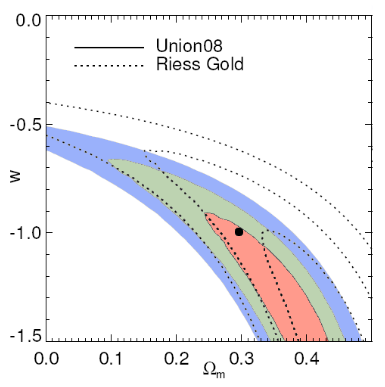
\includegraphics[width=\linewidth]{figures/chapter5/fig5.8.png}
\end{minipage}
\hfill
\begin{minipage}[c]{0.48\textwidth}
  \caption{Comparison of the $(\Omega_M , w_0)$ credible regions from the Union and Gold (Riess) data modified from \cite{Kowalski2008}. I have coloured the image for better contrast: red, green and blue filled contours show $1, 2, 3\sigma$ regions from the Union set and the empty contours the Gold set. I also added a dot to show the position of the $\Lambda$CDM model. Image credit: Fig. 13 from \cite{Kowalski2008}.}
  \label{fig:fig5.8}
\end{minipage}
\end{figure}

\begin{figure}
\centering
\begin{minipage}[c]{0.48\textwidth}
  \centering
  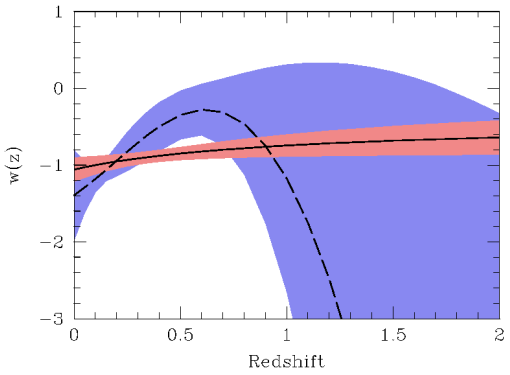
\includegraphics[width=\linewidth]{figures/chapter5/fig5.9.png}
\end{minipage}
\hfill
\begin{minipage}[c]{0.48\textwidth}
  \caption{$90\%$ confidence limits on $w(z)$ for the linear parameterisation $w(z) = w_0 + w_1 \frac{z}{1+z}$ (red) and a quartic polynomial $\sum_{i=0}^{4} w_i (\ln{}(1 + z))^{i} $ (blue) using the Gold set. The best-fit equations of state are the black lines: solid for the linear parameterisation and dashed for the polynomial.  Image credit: Fig. 10 in \cite{Riess2007}.}
  \label{fig:fig5.9}
\end{minipage}
\end{figure}


The two-dimensional models illustrate degeneracies between the different parameters. This causes difficulty if one wishes to estimate the cosmological parameters from Ia SNe alone: the data is sufficient to constrain the parameters pairwise, but insufficient to determine a value for them separately. Linear degeneracy clearly exists for the pairs $(\Omega_m , \gamma)$ (\cref{fig:fig5.4}), $(w_0 , w_1 )$ (\cref{fig:fig5.5}), whereas the other four combinations $(\Omega_m , w_0)$ (\cref{fig:fig5.2}), $(\Omega_m , w_1 )$ (\cref{fig:fig5.3}), $(w_0 , \gamma)$ (\cref{fig:fig5.6}), $(w_1 , \gamma)$ (\cref{fig:fig5.7}) display degeneracies which have a more complex curved shapes. These shapes are linear for intermediate values of the parameters, however they curve to become horizontal or vertical at either end of the credible regions.  In these locations the parameters are completely non-degenerate: a precise value for one parameter contributes no information about the value of the other. Despite this, the reduced-error and Snap sets suggest linear degeneracy may emerge from these credible regions if the distance modulus uncertainties are reduced.

The $(\Omega_m , w_0)$ credible regions replicate the results from the SNe search teams for the three observational sets. In particular \cite{Kowalski2008} confirms the discrepancy (\cref{fig:fig5.8}) I found between the Gold (\cref{fig:fig5.2}c) and Union (\cref{fig:fig5.2}b) samples. 
The $\Lambda$CDM model falls in the 1$\sigma$ region for both Constitution (\cref{fig:fig5.2}a) and Union sets, whereas it is more unlikely to be predicted from the Gold data, as it lies in the 2$\sigma$ region. The smaller-error sets have 3$\sigma$ regions which rule out the $\Lambda$CDM values and are entirely enclosed by the 1$\sigma$ regions from the respective observational sets, with the ratio of areas within 1$\sigma$ indicating a better-than-linear scaling relationship between uncertainties in $\mu(z)$ and uncertainties in the values of the cosmological parameters. The dots at the position of the $\Lambda$CDM parameter values show that only the Constitution set favour the concordance model, whereas the Union set places it at the $1-2\sigma$ boundary and the Gold set firmly in the 2$\sigma$ credible region. 
In comparison to the Constitution set, the Union set favours more negative values of the constant equation of state parameter $w_0$ for equivalent values of the fractional matter density $\Omega_m$ whereas the Gold set favours more negative $w_0$ and larger values of $\Omega_m$ . There is overlap between the 1$\sigma$ credible regions for the observational sets, however this region does not include the concordance model.

Including a time-varying equation of state 
\begin{equation*}
w(z) = \Lambda + w_1 \frac{z}{1+z} = -1 + w_1 \frac{z}{1+z}    
\end{equation*}
produces the credible regions for $(\Omega_m , w_1)$, which do not favour the $\Lambda$CDM model. 
The Constitution data (\cref{fig:fig5.4}a) places the $\Lambda$CDM parameter values at the $1 - 2\sigma$ boundary, the Gold data in the 2$\sigma$ region and the Union data at the $2-3\sigma$ region boundary, while the reduced-error sets all place $(\Omega_m , w_1) = (0.3, 0)$ outside 3$\sigma$. 
At first glance, this strongly suggests that a negative time variation in $w(z)$ is far more likely than a constant. However, this result may simply be a consequence of fixing $w_0$ at a value which does not produce a good fit to the data,\footnote{This is seen by the intersection of $w_0 = -1$ (and $w_1 = 0$ because it is fixed) with the $(\Omega_m , w_0)$ credible regions, discussed in the previous paragraph.} which causes the $w_1$ value to decrease in an attempt to improve the fit. This is supported by the degeneracy between the two parameters in the dark energy equation of state shown in the $(w_0 , w_1)$ credible regions. A model varying the fractional matter density and both equation of state parameters is necessary to gain more insight into this problem.

Next we examine the linear $(w_0 , w_1)$ correlation (Fig. ??). One may question whether this is a consequence of the equation of state constraints or truly a product of the available data. Although a flat prior was assumed for all of the parameter values, the form of the dark energy equation of state 
\begin{equation*}
    w(z) = w_0 + w_1 \frac{z}{1+z} 
\end{equation*}
acts as a strong prior, placing (perhaps unjustifiably) strong constraints on the behaviour of $w(z)$. \cref{fig:fig5.9} demonstrates this by plotting the 95\% credible region (2$\sigma$ confidence $z$ limits) on $w(z)$ for the linear parameterisation 
\begin{equation*}
    w(z) = w_0 + w_1 \frac{z}{1+z} 
\end{equation*}
(red) and a quartic polynomial 
\begin{equation*}
    w(z) = \sum_{i=0}^{4} w_i \left[ \ln(1+z) \right]^i
\end{equation*}
(blue) using the Gold set \cite{Riess2007}. The behaviour of the best-fit models for the dark energy equation of state 
differs dramatically: the linear parameterisation is (by definition) monotonically increasing as $z \rightarrow{} \infty{}$, however the quartic admits a non-monotonic evolution with recent changes (at $z < 0.1$) in $w(z)$. This suggests that the linear parameterisation generates artificially well-constrained results for w(z). Conversely, one may argue that the use of the more general equation of state is unwarranted (it merely expresses our gross ignorance, rather than being physically well-motivated,so the results may depend strongly upon the choice of prior \cite{Efstathiou2008}), as the Gold set does not have sufficient SNe (only 23 at $z > 1$) \cite{Riess2007} to place limits on such a general w(z). This problem may be resolved by using the $> 1000$ samples expected from observations with survey telescopes such as SNAP/WFIRST, the Large Synoptic Survey Telescope\footnote{LSST \url{http://www.lsst.org}} and the Panoramic Survey Telescope and Rapid Response System\footnote{Pan-STARRS \url{http://pan-starrs.ifa.hawaii.edu/public}} \cite{Leibundgut2008}. These projects will provide large, homogeneous data sets with increased numbers of SNe at z > 1, which will give tighter constraints on $w(z)$ at (relatively) high redshift \cite{Leibundgut2008}.

Finally we analyse the credible regions including interaction, for which there are no existing results from the SNe survey teams. The ($\Omega_m$ , $\gamma$) models show a linear correlation between the fractional matter density and the interaction parameter. Both the Constitution (\cref{fig:fig5.4}a) and Union (\cref{fig:fig5.4}b) sets suggest that the concordance model is plausible, since ($\Omega_m$ , $\gamma$) = (0.3, 0) lies within the 1$\sigma$ regions, however the Gold data once again disagrees, placing it only within 2$\sigma$. The Constitution 0.2x set also favours the $\Lambda$CDM model, however the Gold 0.2x and Union 0.2x sets neither agree well with $\Lambda$CDM nor their normal-error counterparts (the 1$\sigma$ regions intersect the 2 and 3$\sigma$ region of the normal-error sets). 
This is probably caused by a convergence problem with the Markov chains: both of these data–model combinations had to be run for unusually large step sizes before the resulting histogram was smooth, but they may have needed even longer before the histogram converged to the posterior. Highly negative values of $\gamma$ represent transfer of energy from matter into dark energy, resulting in $\Omega_m \rightarrow{} 0$ as $z \rightarrow{} -1$. As this result is not indicated by the observational data, these two results remain a curiosity. Overall, $\gamma$ = 0 lies within the 1$\sigma$ regions for values of $\Omega_m$ which are observationally likely, (0.25 . $\Omega_m$ . 0.5), so at this stage no interaction remains a probable result. 
The credible regions for ($w_0$ , $\gamma$) (\cref{fig:fig5.6}) and ($w_1$ , $\gamma$) (\cref{fig:fig5.7}) have degeneracies which are unlikely to be resolved. This is because the interaction in the adiabatic Friedmann equation \cref{eq:1.10} can be represented as an effective non-constant equation of state [3, 67], which contributes an additional term to w(z). As $\gamma \rightarrow{} -1$ it loses its degeneracy with $w_1$ : the credible regions (\cref{fig:fig5.7}) become horizontal, so a particular value for $\gamma$ places no constraint upon the value for $w_1$ . At the limit:

\begin{subequations}
\label{eq:5.1}
\begin{align}
    \frac{\dd{\Omega}_{m}}{\dd{z}} &=
    \frac{1}{1+z} \left(
        3 \Omega_{m} + \frac{1}{H(z)}
    \right)
    \label{eq:5.1a} \\
    \frac{\dd{\Omega}_{X}}{\dd{z}} &=
    \frac{1}{1+z} \left(
        3 \Omega_{X} \left(
            1 + w_{0} + w_{1} \frac{z}{1+z}
        \right)
        - \frac{1}{H(z)}
    \right)
    \label{eq:5.1b}
\end{align}
\end{subequations}

so in the past, as $z \rightarrow{} \infty{}$, the effect of $H(z)$ will swamp the effect of any values of $w(z)$ and the value of $\Omega_X$ will be negative,\cite{vanOsten2006} which is physically impossible (as it is a fractional density). The credible regions \cref{fig:fig5.2,fig:fig5.3,fig:fig5.4,fig:fig5.5,fig:fig5.6,fig:fig5.7} show that a large section of the 2d parameter space often lies within the 1$\sigma$ credible region, illustrating that the Friedmann equations may produce exceedingly similar distance modulus curves for very different initial conditions (fits to the data are given in §B). Therefore one must look for other observational data which does not display the same degeneracy\footnote{This statement is true only for $\Lambda$CDM-based models with a dark energy equation of state based on a barotropic model. More exotic possibilities such as the ”doomsday” and braneworld models do not display opposing degeneracies: see \cite{Rubin2008} for a summary of SN+\cmb{}+\bao{} credible regions with more exotic models.} in order to obtain tight constraints (on the order of those for the one-parameter models). 
Fortunately, the two other sources used for cosmological parameter estimation are complementary to SNe: both the \cmb{} and \bao{} display the opposite degeneracy (see \cref{sec:5.3}), at least for $\Omega_m$ , $w_0$ and $w_1$. It remains to be seen whether similar relationships exist for $\gamma$.





